\section{Method}\label{s:method}
\begin{figure*}
  \centering
  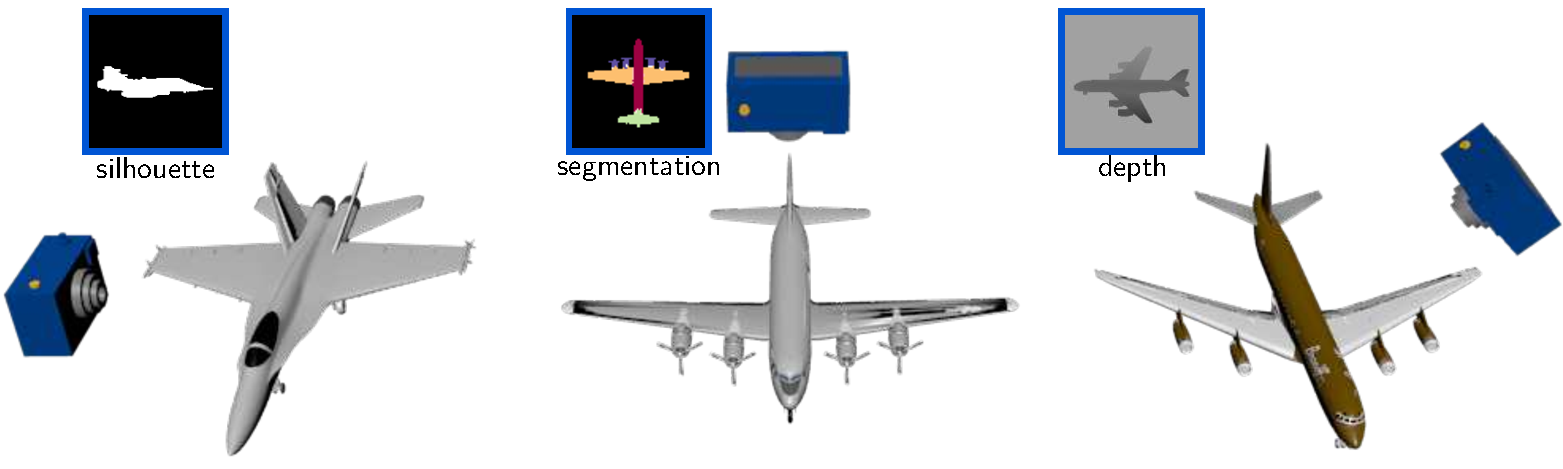
\includegraphics[width=0.85\linewidth]{fig/projections.pdf}
  \caption{\label{fig:projection} 
    The input to our model consists of multiple renderings of
    different objects taken from different viewpoints.
    Those image are \emph{not} annotated with identification or viewpoint information.
    Our model is able to handle images from objects rendered as
    silhouettes (left), semantic segmentation maps (middle) or
    depth maps (right).
}
\vspace{-8pt}
\end{figure*}


Our method builds upon GANs proposed in
Goodfellow~\etal~\cite{goodfellow2014generative}.
The goal of a GAN is to train a generative model in an
adversarial setup.
The model consists of two parts: a \emph{generator} and a
\emph{discriminator}.
The generator $G$ aims to transform samples drawn from a simple
distribution ${\cal P}$ that appear to have been sampled from the
original dataset.
The discriminator $D$ aims to distinguish samples generated
by the generator from real samples (drawn from a data distribution
${\cal D}$).
Both the generator and the discriminator are trained jointly by
optimizing:

\begin{equation}\label{eqn:gan}
\min_{G}\max_{D} \mathbb{E}_{x\sim{\cal D}} [ \log \left(D(x)\right) ] + \mathbb{E}_{z\sim{\cal P}} [ \log \left(1-D(G(z))\right)].
\end{equation}

Our main task is to train a generative model for 3D shapes without
relying on 3D data itself, instead relying on 2D images from those shapes, without
any view or shape annotation\footnote{We later relax this assumption
  to incorporate extra supervision.}.
In other words, the data distribution consists of 2D images taken from
different views and are of different objects.
To address this mismatch we factorize the 2D image generator into a 3D
shape generator (${\cal G}_{3D}$), viewpoint generator $(\theta,\phi)$, and a
projection module ${\cal P_{\theta,\phi}}$ as seen in Figure~\ref{fig:prgan-arch}.
The challenge is to identify a representation for a diverse set of shapes
and a differentiable projection module to create final 2D images and
enable end-to-end training. 
We describe the architecture employed for each of these next. 

\paragraph{3D shape generator ($G_{3D}$).}
The input to the entire generator is $z \in \mathbb{R}^{201}$ with
each dimension drawn independently from a uniform distribution
$\text{U}(-1,1)$.
Our 3D shape generator ${\cal G}_{3D}$ transforms the first 200 dimensions of $z$ to a
$N\times N \times N$ voxel representation of the shape.
Each voxel contains a value $v\in[0, 1]$ that represents its occupancy.
The architecture of the 3D shape generator is inspired by the
DCGAN~\cite{radford2015unsupervised} and 3D-GAN~\cite{wu2016learning}
architectures. 
It consists of several layers of 3D convolutions, upsampling, and
non-linearities, as shown in Figure~\ref{fig:prgan-arch}.
The first layer transforms the 200 dimensional vector to a $256\times
4 \times 4 \times 4$ vector using a fully-connected layer.
Subsequent layers have batch normalization and ReLU layers between them
and use 3D kernels of size $5\times5\times5$.
At every layer, the spatial dimensionality is increased by a factor of 2 and
the number of channels is decreased by the same factor, except for the last layer whose
output only has one channel (voxel occupancy).
The last layer is succeeded by a sigmoid activation instead of a ReLU in order
to keep the occupancy values in $[0,1]$.

\paragraph{Viewpoint generator $(\theta,\phi)$.}
The viewpoint generator takes the last dimension of $z \in
\text{U}(-1,1)$ and transforms it to a viewpoint vector
$(\theta,\phi)$.
The training images are assumed to have been generated from 3D models
that are upright oriented along the y-axis and are centered at the
origin.
Most models in online repositories and the real world satisfy this
assumption (\eg, chairs are on horizontal planes).
We generate images by sampling views uniformly at random from one of
eight pre-selected directions evenly spaced around the y-axis (\ie,
$\theta=0$ and $\phi=0^\circ$, $45^\circ$, $90^\circ$, $...$, $315^\circ$), as seen
in Figure~\ref{fig:projection}.
Thus the viewpoint generator picks one of these directions uniformly
at random.


\paragraph{Projection module ($Pr$).}
The projection module $Pr$ renders the 3D shape from the given
viewpoint to produce an image. 
For example, a silhouette can be
rendered in the following steps.
The first step is to rotate the voxel grid to the corresponding viewpoint.
Let $V : \mathbb{Z}^3 \rightarrow [0,1] \in \mathbb{R}$ be the voxel grid, a function that
given an integer 3D coordinate $c=(i,j,k)$ returns the occupancy of the voxel centered at $c$.
The rotated version of the voxel grid $V(c)$ is defined as 
$V_{\mathbb{\theta, \phi}} = V(\lfloor{R(c, \mathbf{\theta,\phi})}\rfloor)$,
where $R(c, \mathbf{\theta},\phi)$ is the coordinate obtained by rotating $c$ around the origin
according to the spherical angles $\mathbf{(\theta,\phi)}$. 
Notice that $R$ is straightforwardly implemented as a matrix multiplication and can be
extended to model other types of transformations, \eg~perspective transformations.
Refer to the Appendix A in~\cite{yan2016perspective} for more details.

The second step is to perform the projection to create an image from
the rotated voxel grid.
This is done by applying the projection operator 
$Pr((i,j),V) = 1 - e^{-\sum_{k}V(i,j,k)}$. 
Intuitively, the operator sums up the voxel occupancy values along
each line of sight (assuming orthographic projection), and applies
exponential falloff to create a smooth and differentiable
function.
When there is no voxel along the line of sight, the value is
0; as the number of voxels increases, the value approaches 1.
Combined with the rotated version of the voxel grid, we define our
final projection module as:
$Pr_{\theta,\phi}((i,j),V) = 1 - e^{-\sum_{k}V_{\theta,\phi}(i,j,k)}$. 
As seen in Figure~\ref{fig:projection} the projection module can well
approximate the rendering of a 3D shape as a binary silhouette image,
and is differentiable.
Section~\ref{s:discussion} presents projection modules that
render the shape as a depth image or one labeled with part segmentations
using similar projection operations, as seen in Figure~\ref{fig:projection}. 
Thus the 2D image generator $G_{2D}$ can be written compositionally as
${G}_{2D} = {Pr}_{(\theta, \phi)} \circ G_{3D}$.



\paragraph{Discriminator ($D_{2D}$).}
The discriminator consists of a sequence of 2D convolutional layers with
batch normalization layer and LeakyReLU activation~\cite{maas2013rectifier} between them. 
Inspired by recent work~\cite{radford2015unsupervised,wu2016learning}, we employ
multiple convolutional layers with stride 2 while increasing the
number of channels by 2, except for the first layer,
whose input has 1 channel (image) and output has 256.
Similar to the generator, the last layer of the discriminator is
followed by a sigmoid activation instead of a LeakyReLU.


\paragraph{Training details.}
The entire architecture is trained by optimizing the objective in Equation~\ref{eqn:gan}.
Usually, updates to minimize each one of the losses is applied once at each
iteration.
However, in our model, the generator and the discriminator have a considerably different
number of parameters, as the generator is trying to create 3D shapes,
while the discriminator is trying to classify 2D images.
To mitigate this issue, we employ an adaptive training strategy.
At each iteration of the training, if the discriminator accuracy is higher than 75\%,
we skip its training.
We also set different learning rates for the discriminator and the generator:
$10^{-5}$ and $0.0025$, respectively.
Similarly to the DCGAN architecture \cite{radford2015unsupervised}, we
use ADAM with $\beta_1=0.5$ for the optimization.


